\documentclass{seminar}
%==============================================================================
\usepackage{fancybox}
\usepackage{semcolor}
\usepackage{semlayer}
\usepackage{sem-a4}
\usepackage{epsfig}
\usepackage{subfigure}
\usepackage{amssymb}
%==============================================================================
%COLORS: black,darkgray,gray,lightgray,white,red,green,blue,yellow,cyan,magenta
%==============================================================================
\newcommand{\LG}{\lightgray}
%==============================================================================
% For Black and White slides uncomment the following
%---------------------------------------------------
\renewcommand{\red}{\black}
\renewcommand{\blue}{\black}
\renewcommand{\gray}{\black}
\renewcommand{\green}{\black}
\renewcommand{\magenta}{\black}
\renewcommand{\darkgray}{\black}
%% \newcommand{\openpagina}{\begin{slide} ---------------------------------------------------------------------\\ ~\\  ---------------------------------------------------------------------\\ ~\\  ---------------------------------------------------------------------\\ ~\\  ---------------------------------------------------------------------\\ ~\\  ---------------------------------------------------------------------\\ ~\\  ---------------------------------------------------------------------\\ ~\\  ---------------------------------------------------------------------\\ ~\\   ---------------------------------------------------------------------  \end{slide}}

\newcommand{\openpagina}{}

% ==============================================================================
%==============================================================================

\def\printlandscape{\special{landscape}}    % Works with dvips.

% \slideframe{Oval}

% \onlyslides{1-30}

\overlaystrue
\printlandscape


\begin{document}

\begin{slide}

{\bf Myhill-Nerode verstaan: 3 ingredi\"{e}nten}

\begin{itemize}
\item 
van DFA voor L naar partitie met MN(L)-eigenschappen

\item 
van partitie met  MN(L)-eigenschappen naar DFA voor L

\item 
equivalentierelaties en partities: 2 zichten op 1 concept
\begin{itemize}
\item[] {\footnotesize heeft niks met MN te maken !}

\end{itemize}


\end{itemize}

\end{slide} \openpagina

\begin{slide}

{\bf Van DFA naar partitie van $\Sigma^*$ - voorbeeld I}

Taal L = gegeven door $a^*$ over alfabet $\{a,b\}$




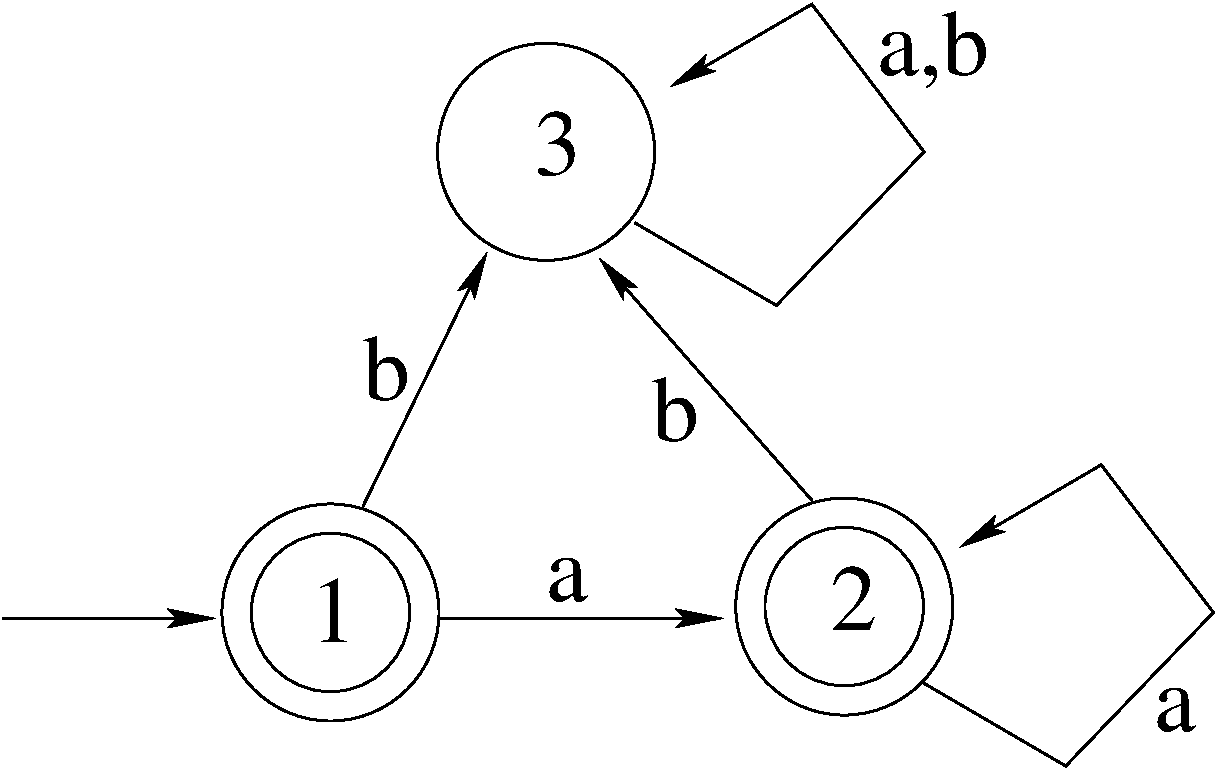
\includegraphics[%
  width=0.25\linewidth,
  keepaspectratio]{mn1.eps}


\begin{itemize}
\item alle strings waarmee je in toestand 1 kan aankomen: $S_1 = \{\epsilon\}$
\item in toestand 2: $S_2 = \{aa^*\}$
\item in toestand 3: $S_3 = \{s|s \in \Sigma^*~en~s~bevat~een~b\}$
\item $S_i = reach(i)$
\end{itemize}

$\{S_1,S_2,S_3\}$ is een eindige partitie van $\Sigma^*$

$\{S_1,S_2,S_3\}$ is fijner dan $\{L, \overline{L}\}$

de equivalentierelatie bepaald door ... is rechts-congruent

\end{slide} \openpagina

\begin{slide}
{\bf $\{S_1,S_2,S_3\}$ en rechts-congruent ...}

neem twee verschillende strings $s_1$ en $s_2$ uit $S_2$
\begin{itemize}
\item in welke set(s) zitten $s_1a$ en $s_2a$ ?
\item in welke set(s) zitten $s_1b$ en $s_2b$ ?
\end{itemize}

neem twee verschillende strings $s_1$ en $s_2$ uit $S_3$
\begin{itemize}
\item in welke set(s) zitten $s_1a$ en $s_2a$ ?
\item in welke set(s) zitten $s_1b$ en $s_2b$ ?
\end{itemize}

% dus:
% \begin{itemize}
% \item 
% $\forall s_1, s_2, x: s_1 \sim s_2 \rightarrow s_1x \sim s_2x$

% \end{itemize}


\end{slide} \openpagina

\begin{slide}

{\bf Van DFA naar partitie van $\Sigma^*$ - voorbeeld II}

Taal L = gegeven door $a^*$ over alfabet $\{a,b\}$




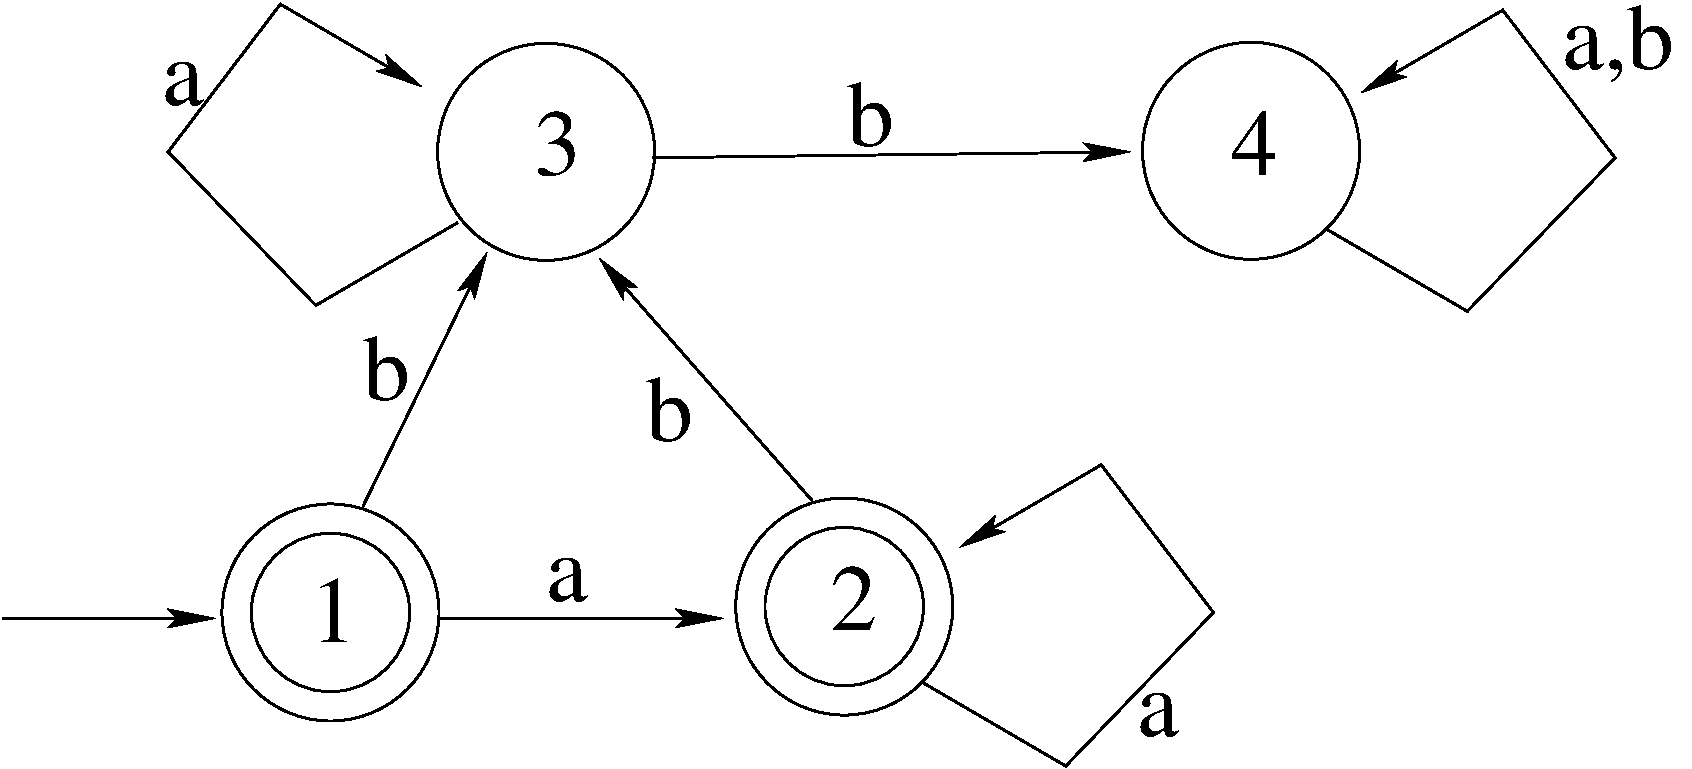
\includegraphics[%
  width=0.3\linewidth,
  keepaspectratio]{mn2.eps}


\begin{itemize}
\item $S_1 = \{\epsilon\}$  en $S_2 = \{aa^*\}$ (zoals in I)

\item $S_3 = \{s|s \in \Sigma^*~en~s~bevat~juist~1~b\}$

\item $S_4 = \{s|s \in \Sigma^*~en~s~bevat~minstens~2~b's\}$

\end{itemize}

$\{S_1,S_2,S_3,S_4\}$ is een eindige partitie van $\Sigma^*$

$\{S_1,S_2,S_3,S_4\}$ is fijner dan $\{L, \overline{L}\}$

de equivalentierelatie bepaald door ... is rechts-congruent

\end{slide} \openpagina

\begin{slide}
{\bf $\{S_1,S_2,S_3,S_4\}$ en rechts-congruent ...}

neem twee verschillende strings $s_1$ en $s_2$ uit $S_2$
\begin{itemize}
\item in welke set(s) zitten $s_1a$ en $s_2a$ ?
\item in welke set(s) zitten $s_1b$ en $s_2b$ ?
\end{itemize}

neem twee verschillende strings $s_1$ en $s_2$ uit $S_3$
\begin{itemize}
\item in welke set(s) zitten $s_1a$ en $s_2a$ ?
\item in welke set(s) zitten $s_1b$ en $s_2b$ ?
\end{itemize}

neem twee verschillende strings $s_1$ en $s_2$ uit $S_4$
\begin{itemize}
\item in welke set(s) zitten $s_1a$ en $s_2a$ ?
\item in welke set(s) zitten $s_1b$ en $s_2b$ ?
\end{itemize}

\end{slide} \openpagina

\begin{slide}
{\bf rechts-congruent betekent}

\begin{itemize}
\item
als $s_1$ en $s_2$ in $S_i$ zitten, dan zitten
          $s_1x$ en $s_2x$ in dezelfde $S_j$ voor alle $x \in \Sigma$

\item 
als $s_1 \sim s_2$ dan $s_1x \sim s_2x$ voor alle $x \in \Sigma$
\end{itemize}

{\bf verband partitie $\{S_1, ..., S_n\}$ en de ge\"induceerde equivalentierelatie}

$s_1 \sim s_2$ als en slechts als $s_1~en~s_2 \in~zelfde~S_i$
\end{slide} \openpagina


\begin{slide}
{\bf Van partitie naar DFA - voorbeeld III}

\begin{itemize}
\item $S_1 = \{\epsilon\}$
\item $S_2 = \{a\}$
\item $S_3 = \{aa\}$
\item $S_4 = \{aaaa^*\}$ (minstens 3 a's en enkel a's)
\item $S_5 = \{a^*ba^*\}$ (juist 1 b)
\item $S_6 = \{a^*ba^*b(a|b)*\}$ (minstens 2 b's)
\end{itemize}

laat L gelijk zijn aan $a^*$

verfijnt $\{L, \overline{L}\}$ - rechts-congruent - eindig

de equivalentierelatie door $\{S_1,S_2,S_3,S_4,S_5,S_6\}$
ge\"induceerd is dus een MN(L)-relatie

\end{slide} \openpagina

\begin{slide}
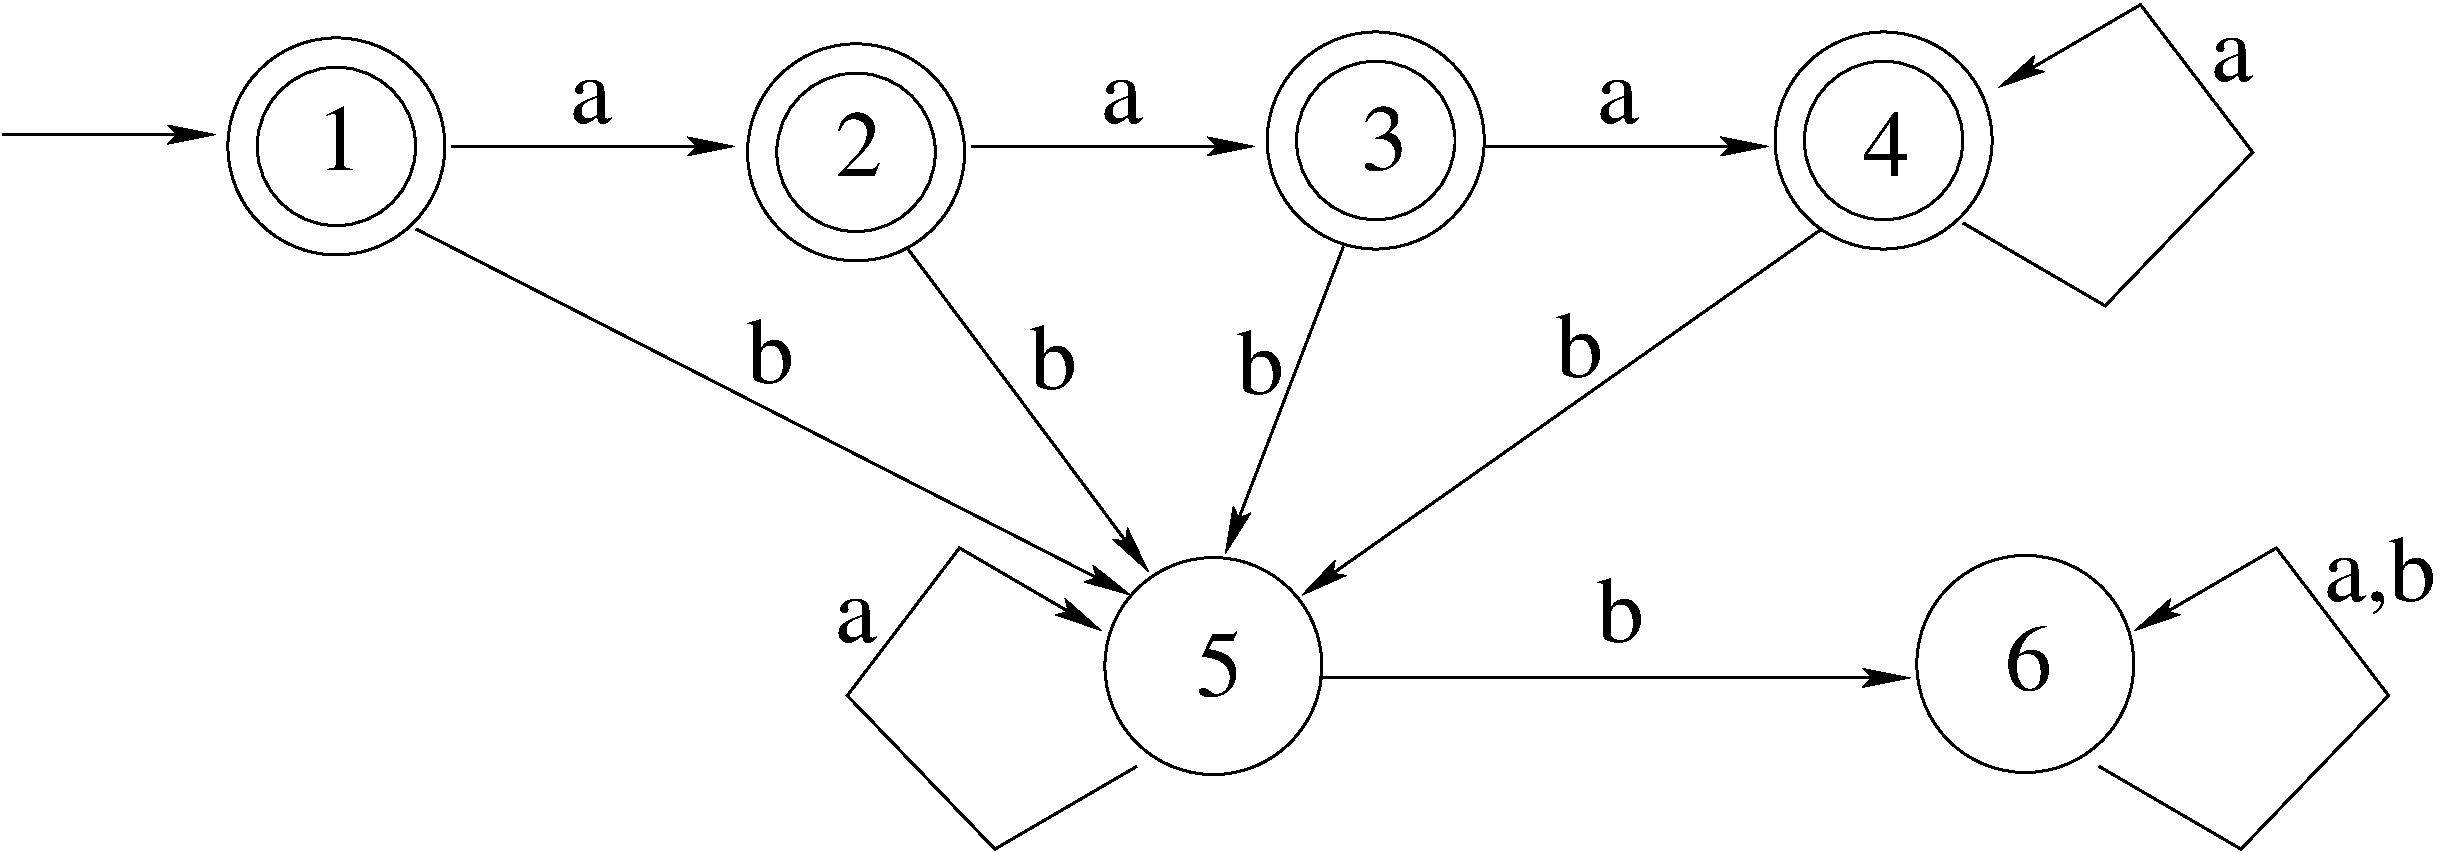
\includegraphics[%
  width=0.8\linewidth,
  keepaspectratio]{mn3.eps}

\vspace{1cm}
welke toestanden zijn accepterend ? waarom ?
\end{slide} \openpagina

\begin{slide}
{\bf Verband tussen MN(L)-relatie en DFA voor L - informeel}

\begin{itemize}
\item met een MN(L)-relatie R1 komt een partitie P1 van $\Sigma^*$ overeen
\item met die partitie P1 komt een DFA1 overeen die L accepteert
\item met DFA1 komt een 
\begin{itemize}
\item partitie P2 overeen en P1 == P2
\item MN(L)-relatie R2 overeen: R1 == R2
\end{itemize}
\item met P2 komt een DFA2 overeen die L accepteert: DFA1 is gelijk
aan DFA2 op een isomorfisme na (hernoeming van de toestanden)
\end{itemize}

daarmee is die cirkel rond\
\end{slide} \openpagina

\begin{slide}
{\bf Van MN(L)-relatie naar DFA voor L}

\begin{itemize}
\item met een MN(L)-relatie R komt een partitie $P = \{S_1,...,S_n\}$ van
$\Sigma^*$ overeen
\item met elke $S_i$ komt een toestand $q_i$ overeen
\begin{itemize}
\item[] {\footnotesize $reach(q_i)$ geeft exact $S_i$}
\end{itemize}
\item $q_i \in F$ alss $S_i \subseteq L$ (P verfijnt $\{L,\overline{L}\}$)
\item $q_s$ komt overeen met de $S_i$ waartoe $\epsilon$ behoort

\item de rechts-congruentie dient om $\delta$ correct te defini\"eren:
\begin{itemize}
\item[] $\delta(q_i,a)$ is ... neem gelijk welke (*) $s \in S_i$, neem de
$S_j$ waartoe $sa$ behoort, dan is $\delta(q_i,a) = q_j$
\item[] (*) werkt wegens de rechts-congruentie
\end{itemize}

\end{itemize}



\end{slide} \openpagina

\begin{slide}
{\bf Van DFA voor L naar MN(L)-relatie}

\begin{itemize}
\item definieer: $S_i$ gelijk aan $reach(q_i)$
\item dan is $P = \{S_1,...,S_n\}$ een partitie van $\Sigma^*$
\begin{itemize}
\item P is eindig
\item P is rechts-congruent
\item P verfijnt $\{L,\overline{L}\}$ - d.w.z. elke $reach(q_i)$ is deel
van $L$ of van $\overline{L}$
\end{itemize}
dus P induceert een MN(L)-relatie
\end{itemize}

\end{slide} \openpagina

\begin{slide}
{\bf Test ...}

Neem $\Sigma = \{a,b\}$

Is $\{L, \overline{L}\}$ 
\begin{itemize}
\item 
een MN(L)-relatie voor elke reguliere L ?
\item 
een MN(L)-relatie voor sommige reguliere L ?
\item 
een MN(L)-relatie voor welke reguliere L ? 
\end{itemize}

Bestaat er een MN(L)-relatie voor 
\begin{itemize}
\item alle CFLs ?
\item sommige CFLs ?
\item welke CFLs juist ?
\end{itemize}


\end{slide} \openpagina


\begin{slide}
{\bf Twee tralies: equivalentierelaties over X en partities van X}

\begin{itemize}
\item 
een {\bf partitie} van X is een rij van $X_i (\neq \emptyset)$ zodanig dat
\begin{itemize}
\item 
$X_i \subseteq X$
\item 
$\cup_i X_i = X$
\item 
$X_i \cap X_j = \emptyset$ als $i \neq j$
\end{itemize}

\item 
een {\bf equivalentierelatie $\sim$ over X} is een deelverzameling van
$X \times X$ (= de koppels van elementen uit X) zodanig dat
\begin{itemize}
\item 
$\sim$ is reflexief: $x \sim x$ voor alle $x \in X$
\item 
$\sim$ is symmetrisch: $x \sim y$ impliceert $y \sim x$

\item 
$\sim$ is transitief: $x \sim y$ en $y \sim z$ impliceert $x \sim z$

\end{itemize}


\end{itemize}
\end{slide} \openpagina


\begin{slide}

\begin{itemize}
\item 
Als de rij $X_i$ een partitie is van X, dan definieert

$x \sim y$ alss $x$ en $y$ behoren tot dezelfde $X_j$

een equivalentierelatie over X

{\em die equivalentierelatie is ge\"{i}nduceerd door de partitie}


\item 
Als $\sim$ een equivalentierelatie over X is, dan vormen de
equivalentieklassen van X een partitie van X

{\em die partitie is ge\"{i}nduceerd door de equivalentierelatie}

\begin{itemize}
\item[]
{\footnotesize een equivalentieklasse is een maximaal deel D van X zodat alle
  elementen van D equivalent zijn}

\end{itemize}
\end{itemize}


\end{slide} \openpagina

\begin{slide}

\begin{itemize}
\item 
de (eindige) partities van X vormen een tralie
\begin{itemize}
\item 
partiele orde: $\{X_i\}$ is {\em fijner} dan $\{Y_j\}$ indien

elke $X_i$ een deel is van een $Y_j$
\begin{itemize}
\item[] voorbeeld: $X = \{a,b,c,d\}$, dan is

$\{\{a\},\{b\},\{c\},\{d\}\}$ fijner dan $\{\{a,b\},\{c\},\{d\}\}$

\end{itemize}

\item 
grootste (grofste) partitie is \{X\}
\item 
kleinste (fijnste) partitie is \{\{$x_1$\}, \{$x_2$\} ... \} (...)
\end{itemize}

\item 

de equivalentierelaties (met eindige index) vormen een tralie (door
erfenis van hierboven)

\item 
die tralies zijn compleet, t.t.z. (o.a.)
\begin{itemize}
\item 
als $\{X_i\}$ en $\{Y_j\}$ partities zijn, dan bestaat het supremum van
$\{X_i\}$ en $\{Y_j\}$, t.t.z. een fijnste partitie $\{Z_k\}$ zodat

$\{X_i\}$ fijner is dan $\{Z_k\}$ en $\{Y_j\}$ fijner is dan $\{Z_k\}$

\end{itemize}


\end{itemize}

\end{slide} \openpagina

\begin{slide}

{\bf Nog eens het supremum}

\begin{itemize}
\item gegeven twee equivalentierelaties $\sim_1$ en $\sim_2$; dan is
$\sim_{sup}~\triangleq~sup(\sim_1,\sim_2)$ gedefini\"eerd als
\begin{itemize}
\item[] $x \sim_{sup} y$ is de kleinste eqrel die $(x \sim_1 y) \vee (x \sim_2 y)$ bevat
\end{itemize}
$x \sim_{sup} y$ is een equivalentierelatie

\item gegeven twee partities $S = \{S_1,...,S_n\}$ en $T = \{T_1,...,T_m\}$;
dan is $R = sup(S,T)$ een partitie $\{R_1,...,R_l\}$ gedefini\"eerd als ...
\begin{itemize}
\item[] R is de kleinste partitie die S en T bevat
\item[] in het bijzonder: elke $S_i$ zit in een $R_k$; elke $T_i$ zit
in een $R_k$; dus, elke $R_k$ is de unie van een aantal $S_i$ en $T_j$
\end{itemize}

\end{itemize}


\end{slide} \openpagina

\begin{slide}
{\bf Het verband tussen de suprema}

Als S en T twee partities zijn en $\sim_S$ en $\sim_T$ de
ge\"induceerde equivalentierelaties, dan is

\begin{itemize}
\item[]$\sim_{sup(S,T)} == sup(\sim_S,\sim_T)$
\end{itemize}



Omgekeerd: als $\sim_1$ en $\sim_2$ twee equivalentierelaties zijn,
en $S_{\sim_1}$ en $S_{\sim_2}$ zijn de ge\"induceerde partities, dan is

\begin{itemize}
\item[] $\sim_{sup(S_{\sim_1},S_{\sim_2}}) == sup(\sim_1,\sim_2)$
\end{itemize}

\end{slide} \openpagina


\begin{slide}
{\bf De tralie van MN(L)-relaties}

\begin{itemize}
\item een deel-tralie van {\bf alle} relaties (met eindige index)
\item neem twee MN(L)-relaties R1 en R2: sup(R1,R2) is een MN(L)-relatie
\item neem twee DFAs D1 en D2 die zelfde taal accepteren, en neem de
DFA D die komt van
\begin{itemize}
\item neem de MN(L)-relatie R1 van D1
\item neem de MN(L)-relatie R2 van D2
\item neem sup(R1,R2) = R
\item neem de DFA D van R
\end{itemize}
D bepaalt L {\bf en} D heeft {\em niet meer}
toestanden dan D1 en D2
\end{itemize}


\end{slide} \openpagina

\begin{slide}

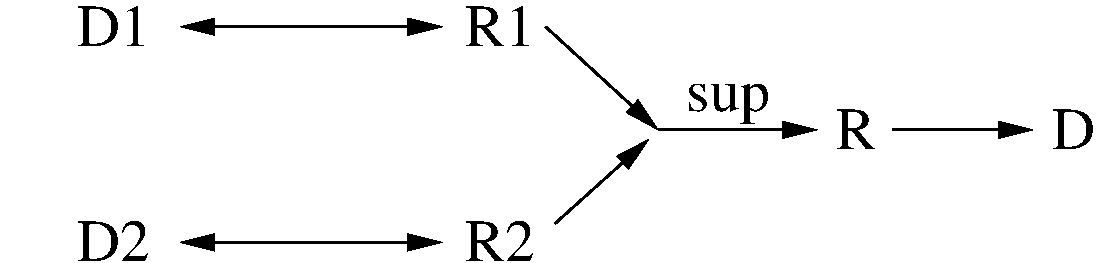
\includegraphics[%
  width=0.8\linewidth,
  keepaspectratio]{mn4.eps}

{\bf De stelling:}
Als D1 en D2 minimale DFAs zijn voor L, dan zijn D1 en D2 isomorf


{\bf $\underline{Bewijs}$}
D is {\em niet groter} dan D1 en D2; als D1 en D2 al minimaal waren, dan
is D isomorf met D1, want R en R1 zijn even groot (als partities) en ook is D isomorf met D2, dus is D1 isomorf met D2
\end{slide} \openpagina


\end{document}
